\documentclass[11pt]{article}
\usepackage{geometry} 
\geometry{a4paper,top=3cm,bottom=3cm,left=2.5cm,right=2.5cm}   
\usepackage{multicol}
\usepackage[english, italian]{babel}
\usepackage{fancyhdr}
\usepackage{fancyvrb}
\usepackage{musicography}
\geometry{centering}
\usepackage{graphicx}
\usepackage{mathpazo} %font
%\usepackage{listings}

%\lstset{size=\tiny}


\pagestyle{fancy}                                 %serve ad inserire la linea sopra e il titolino
\rhead{Lezione 2 "\textit{Programmazione in Faust 2"}}
\renewcommand{\headrulewidth}{5pt} %grandezza della linea in alto
\renewcommand{\footrulewidth}{1pt}   % grandezza della linea in basso


\begin{document}
\begin{minipage}{0.55\linewidth}
\vspace{0.3cm}
\large{\textbf{Gabriele Petrillo}}\\
\end{minipage}

\vspace{0.3cm}
\begin{minipage}{0.95\linewidth}
\begin{center}
\huge{\textbf{Programmazione in Faust 2}} \\
\end{center}
\end{minipage}
\vspace*{0.2cm}


%=========ABSTRACT=======================
\begin{center}
\begin{minipage}[c]{14cm}


\textit{L'obiettivo di questa lezione è conoscere i tipi primitivi di base, la sintassi del linguaggio, la rappresentazioni a blocchi dei programmi, e verranno implementati dei semplici effetti di echo.}

\end{minipage}
\end{center}
\vspace*{0.2cm}

%=========ARTICOLO========================
\setlength{\columnsep}{3em}

\begin{multicols*}{2}
\parskip=0pt

\textbf{I tipi di dato Primitivi}\\

I tipi di dato primitivi possono essere definiti come dei blocchi di base pre-costruiti con cui è possibile costruire programmi complessi.

In Faust sono disponibili 60 operatori primitivi che comprendono operazioni aritmetiche, trigonometriche, di comparazione, ecc. Ad esempio l'operatore primitivo \textit{+} somma due segnali in ingresso e produce un segnale in uscita. \\

\begin{center}
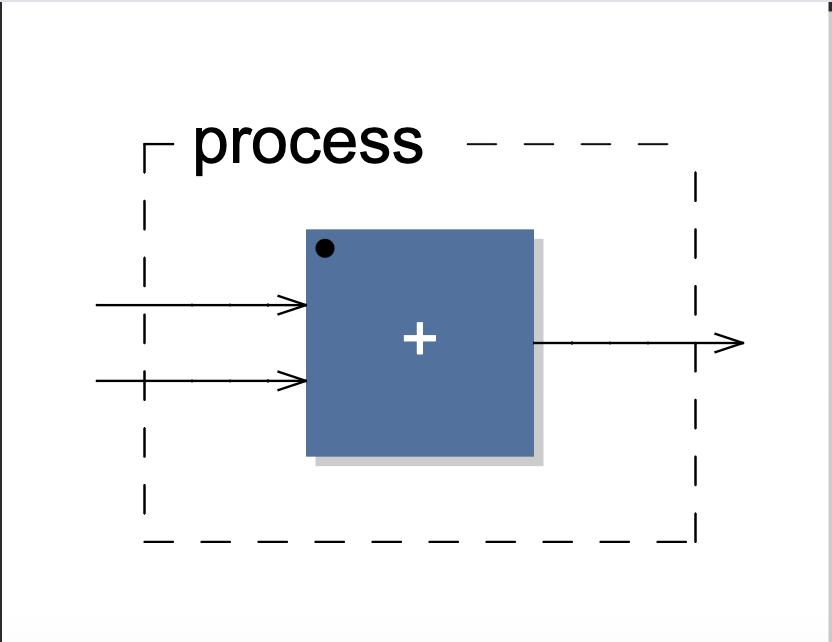
\includegraphics[scale=0.3]{img/01.png}

{\scriptsize \emph{fig.1 }}
\end{center}

La programmazione in Faust consiste essenzialmente nell'assemblare più circuiti audio per costruirne uno più complesso. Per comporre questi circuiti si utilizzano cinque operatori di base che sono ordine:

\begin{enumerate}
\scriptsize
\item A $<$: B - Split; 
\item A :$>$ B - Merge; 
\item A : B - Sequential;
\item A , B - Parallel;
\item A ~ B - Recursion;
\end{enumerate}

Prima di iniziare con tutte queste primitive è importante come rappresentare il segnale audio in Faust. Il simbolo che rappresenta il segnale è \textit{\_} (underscore) infatti se noi scriviamo il seguente codice faremo accedere il microfono del computer direttamente agli altoparlanti:

\begin{Verbatim}[fontsize=\scriptsize]

process = _;

\end{Verbatim}

Per creare un \textit{"cavo stereo"} abbiamo bisogno di implementare due circuiti in parallelo:

\begin{Verbatim}[fontsize=\scriptsize]

process = _ , _ ;

\end{Verbatim}

In Faust ogni canale audio in entrata deve avere un canale audio in uscita, a volte questo può essere un limite, perché potremmo avere bisogno, ad esempio, di tagliare dei segnali audio che non vogliamo utilizzare, per farlo possiamo usare il tipo primitivo \textit{!} (punto esclamativo): 

\begin{Verbatim}[fontsize=\scriptsize]

process = ! , _ ;

\end{Verbatim}

\textbf{UI Widget}\\

Per generare un segnale continuo (DC) in Faust vengono utilizzati i numeri, ad esempio possiamo creare un segnale continuo\footnote{ricordati di spegnere i tuoi altoparlanti o di non accendere il dsp, potresti danneggiare il tuo impianto} del valore di 1:

\begin{Verbatim}[fontsize=\scriptsize]

process = 1 ;

\end{Verbatim}

Tutti i \textit{"UI Widget"} di Faust sono dei generatori di segnale che devono essere moltiplicati al segnale che devono controllare, ad esempio un \textit{buttons} è un oggetto che crea un segnale continuo pari a 1 quando è premuto e 0 quando non lo è, uno \textit{slider} genera un segnale di ampiezza pari all'azione dell'utente e così via. In Faust esistono due tipologie di slider:

\begin{enumerate}
\scriptsize
\item hslider: slider orizzontale; 
\item vslider: slider verticale; 
\end{enumerate}

Sono identici ed hanno la stessa sintassi: nome tra virgolette, valore di partenza, valore minimo, valore massimo e precisione:

\begin{Verbatim}[fontsize=\scriptsize]

process = hslider("nome dell'oggetto", 
	-1, -1, 1, 0.01)  ;

\end{Verbatim}

Se accendiamo il dsp possiamo sentire dei suoni generati muovendo velocemente lo slider, questi piccoli click vengono generati proprio perché effettivamente lo slider è un generatore di segnale e noi stiamo cambiando velocemente il valore di questi campioni.\\

\textbf{Operazioni Aritmetiche}\\

In Faust esistono dei tipi primitivi che implementano tutte le operazioni aritmetiche di base che possono essere applicate ai segnali:

\begin{enumerate}
\scriptsize
\item + = somma; 
\item - = sottrazione; 
\item * = sottrazione; 
\item / = sottrazione; 
\item \% = sottrazione; 
\item $\land$ = elevazione a potenza;
\end{enumerate}

Per esempio proviamo a costruire un semplice controllo del volume assemblando tre tipi primitivi:

\begin{Verbatim}[fontsize=\scriptsize]

process = _ , hslider("gain", 
	0, 0, 1, 0.01) : * ;

\end{Verbatim}

Se vogliamo avere una precisione maggiore possiamo dividere il segnale del nostro slider per 100:

\begin{Verbatim}[fontsize=\scriptsize]

process = _ , (hslider("gain", 
	0, 0, 100, 0.01) / 100) : * ;

\end{Verbatim}

\textbf{Tipologie di Notazione}\\

La scelta di una tipologia di notazione rispetto ad un altra dipende da cosa andiamo a scrivere in relazione ad una maggiore leggibilità del codice, infatti le tipologie di notazione sono completamente identiche:

\begin{Verbatim}[fontsize=\scriptsize]

process = _ , 0.5 : *;  //core Syntex
process = _  * 0.5 ; //Infix Notation
process = *(_ , 0.5) ; //Prefix Notation
process = *( 0.5) ; //Partial Notation

\end{Verbatim}

\textbf{I comparatori}\\

In Faust sono presenti tutti gli operatori di comparazione sui numeri, ma c'è una differenza importante tra comparare numeri e segnali. Se vengono comparati due numeri otteniamo come risultato \textit{Vero} o \textit{Falso}, mentre se compariamo due segnali che evolvono nel tempo otteniamo effettivamente una funzione, quindi dei valori che evolvono nel tempo ottenendo un valore di comparazione istantaneo che è a sua volta un segnale. I comparatori sono:

\begin{enumerate}
\scriptsize
\item $>$ maggiore di; 
\item $>=$ maggiore o uguale di; 
\item == uguale a; 
\item $!=$ diverso da; 
\item $<$  minore di; 
\item $<=$ minore o uguale a;
\end{enumerate}

Proviamo a scrivere un piccolo programma che compara due valori di un oscillatore con la threshold tra zero e uno controllato da uno slider:

\begin{Verbatim}[fontsize=\scriptsize]
import("stdfaust.lib");
process = os.osc(10), vslider("threshold",
	0, 0, 1, 0.01) : > ;

\end{Verbatim}

\textbf{Delay e Funzioni su tabella}\\

In Faust sono presenti quattro primitive relative al tempo:

\begin{enumerate}
\scriptsize
\item mem =  delay di un campione; 
\item @ = delay variabile ; 
\item rdrtable = leggi una tabella; 
\end{enumerate}

Proviamo a ritardare un segnale, nel prossimo esempio prendiamo un segnale continuo (1) e lo ritardiamo di 1 secondo supponendo che stiamo lavorando ad una frequenza di campionamento di 44100 campioni.

\begin{Verbatim}[fontsize=\scriptsize]
import("stdfaust.lib");
process = 1, 44100 : @;

\end{Verbatim}

Se accendiamo il dsp si sentirà un click dopo un secondo ed un click quando spengiamo il dsp perché il segnale sarà troncato. Per evitare questo possiamo creare una funzione che che sottrae al segnale lo stesso segnale ritardato di un campione, in modo da sottrarre al primo campione zero, e al secondo uno: 

\begin{Verbatim}[fontsize=\scriptsize]

import("stdfaust.lib");
dirac = 1 - mem(1);
process = dirac;

\end{Verbatim}

La primitiva \textit{rdtable} ha tre ingressi, il primo è un segnale costante che definisce la grandezza della tabella, il secondo definisce il contenuto della tabella, mentre l'ultimo è un segnale che gestisce gli indici di lettura della tabella. 

\begin{Verbatim}[fontsize=\scriptsize]

import("stdfaust.lib");
dirac = 1 - mem(1);
phase = 1 : +~ _ : %(4096);
process = 4096, dirac, phase  : rdtable;

\end{Verbatim}

\begin{center}
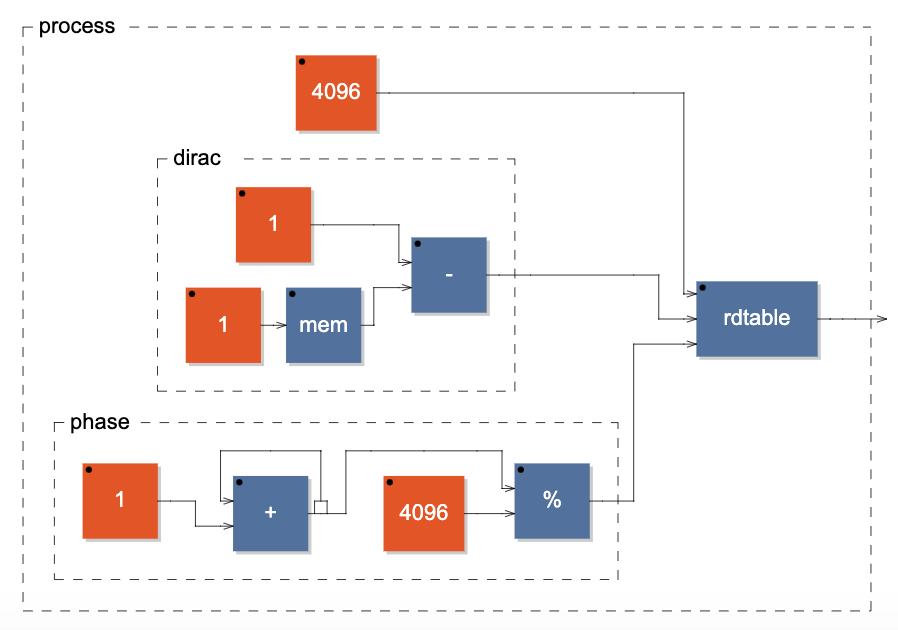
\includegraphics[scale=0.3]{img/05.png}

{\scriptsize \emph{fig.2 }}
\end{center}

La definizione \textit{phase} è una funzione che serve a scorrere tutti gli indici della tabella: abbiamo un segnale di valore 1 che viene sommato a se stesso tramite una funzione ricorsiva. Tutto il blocco viene poi passato ad una funzione modulo(\%) che serve a creare un contatore, infatti si riazzera ogni volta che il totale ha raggiunto 4096 o un suo multiplo, in questo modo si crea un segnale che ciclicamente va da 0 a 4096 leggendo i valori di tutti gli indici della tabella. Abbiamo quindi creato un click ogni 4096 campioni.\\

\textbf{Altri UI utili e i gruppi}\\

Le UI più utili in Faust sono:

\begin{enumerate}
\scriptsize
\item button
\item checkbox ; 
\item nentry;
\item hslider;
\item vslider;
\item hbargraph;
\item nentry o vslider [style: knob];
\end{enumerate}

Prendiamo in considerazione \textit{bargraph}. Questo oggetto ha tre argomenti: l'etichetta, il valore minimo e il valore massimo. Cerchiamo quindi di creare un meter:

\begin{Verbatim}[fontsize=\scriptsize]

import("stdfaust.lib");

meter = _ <: _, display : attach
    with{
        envelop = abs : min(1.00) : 
        	max ~ -(1.0/ma.SR);
        display = envelop :  ba.linear2db :
        	hbargraph("meter", -60, 0);
    };

process = os.osc(440) : _ * 
	hslider("level", 0, 0, 1, 0.001) : 
	meter;

\end{Verbatim}

\begin{center}
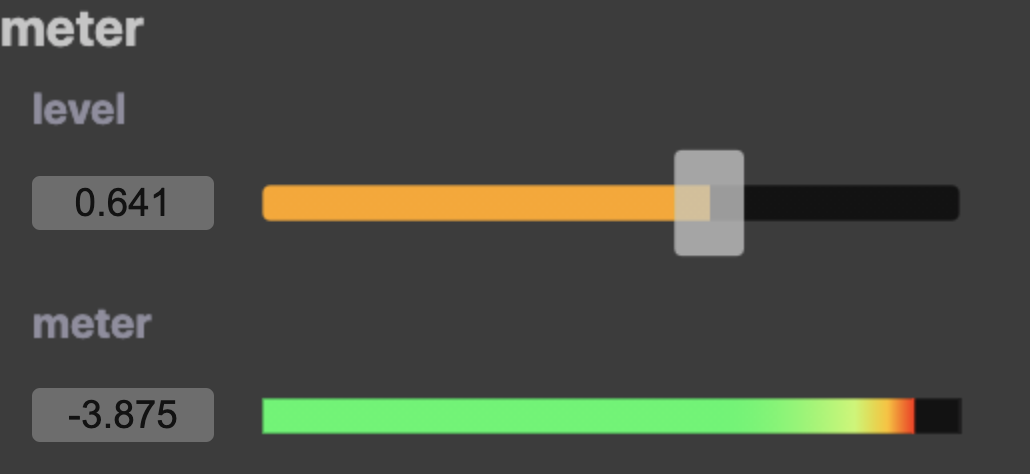
\includegraphics[scale=0.3]{img/06.png}

{\scriptsize \emph{fig.2 }}
\end{center}


Abbiamo costruito un circuito di monitoraggio per un segnale. Questo circuito prende in ingresso un segnale, viene diviso in due segnali uguali tramite la primitiva \textit{attach}, quindi una copia va in un uscita e la seconda all'interno della funzione display. In questa funzione è stato implementato un \textit{envelope follower}.\\

\textbf{La ricorsione}\\

\begin{Verbatim}[fontsize=\scriptsize]
process = _ :+ ~ (_,2:*) ;
\end{Verbatim}

\begin{center}
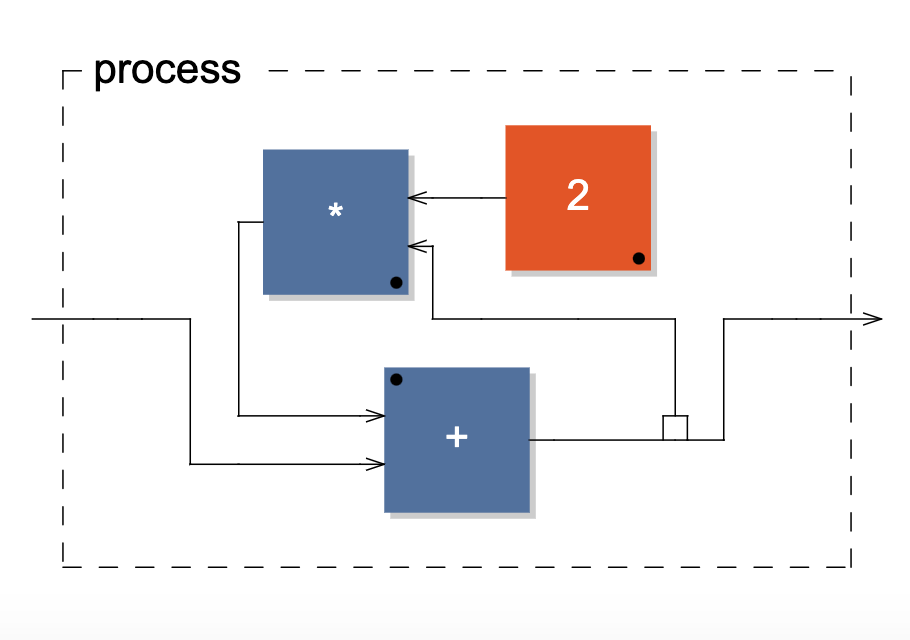
\includegraphics[scale=0.3]{img/02.png}

{\scriptsize \emph{fig.2 }}
\end{center}

\noindent Con un sistema ricorsivo di questo tipo possiamo costruire un generatore di rumore:

\begin{Verbatim}[fontsize=\scriptsize]

random = +(12345) ~ *(1103515245);
noise = random/2147483647.0;
process = noise * 
  vslider("volume[style:knob]", 0, 0, 1, 0.1) <:
   _,_;
\end{Verbatim}

\begin{center}
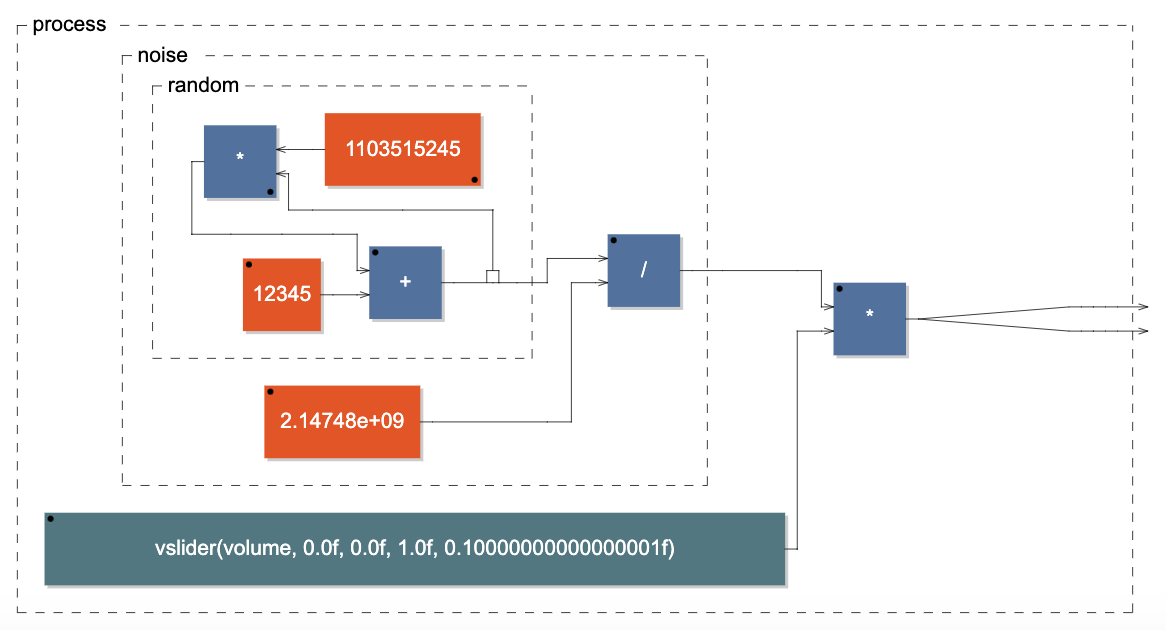
\includegraphics[scale=0.3]{img/03.png}

{\scriptsize \emph{fig.3 }}
\end{center}

\noindent come possiamo vedere dallo schema a blocchi, in maniera ricorsiva andiamo a moltiplicare due numeri in modo da ottenere dei numeri sempre diversi\footnote{i valori usati per questi calcoli sono del tutto casuali}. Successivamente andiamo a scalare questi numeri con una divisione in modo da normalizzare il segnale, infine moltiplichiamo il nostro noise per uno slider in modo da controllarne il volume di uscita.

Con la ricorsione possiamo costruire un effetto \textit{echo}:

\begin{Verbatim}[fontsize=\scriptsize]

import("stdfaust.lib");
echo(d,f) = + ~ (@(d) : *(f));
process = button("play") : 
       pm.djembe(60, 0.3, 0.4, 1) : 
       echo(44100/4, 0.75);
    
\end{Verbatim}

\begin{center}
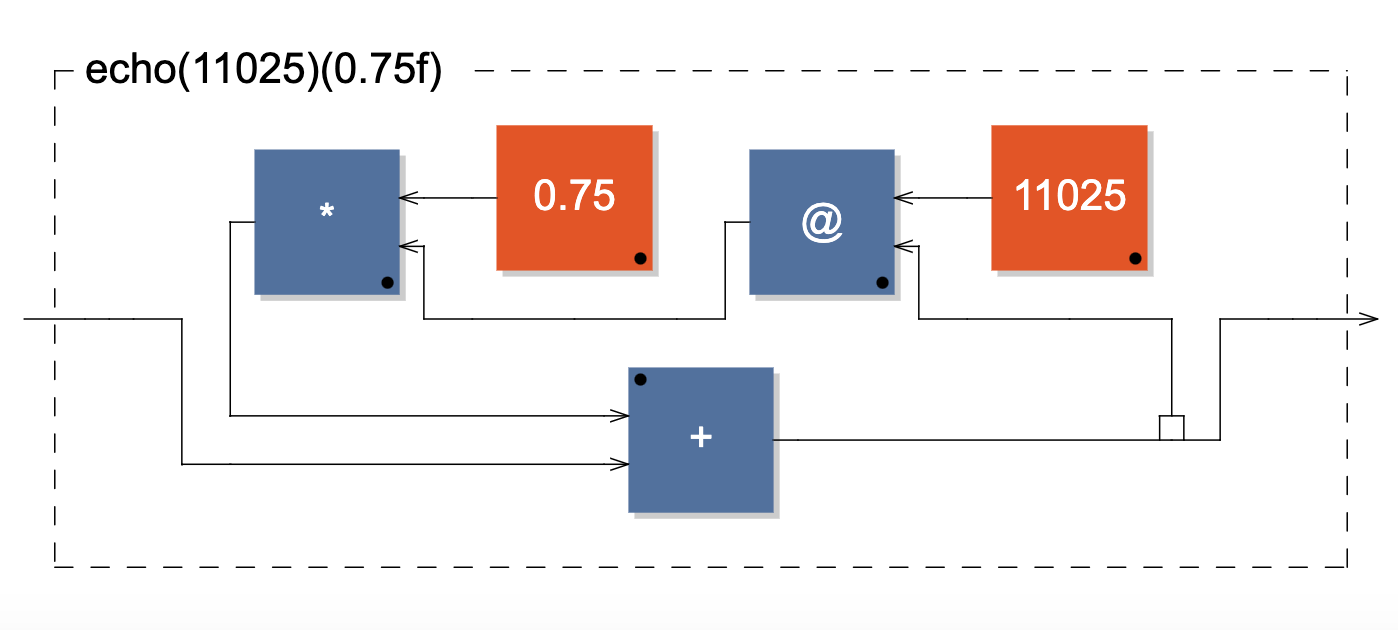
\includegraphics[scale=0.3]{img/04.png}

{\scriptsize \emph{fig.4 }}
\end{center}

Nella prima riga possiamo vedere la definizione della funzione di un echo e tra parentesi abbiamo messo i valori a cui vogliamo avere accesso in questa funzione: il tempo di ritardo in campioni (d) e il moltiplicatore della ricorsione per controllare il feedback (f). Abbiamo quindi l'operatore + che ci serve per sommare il suono diretto con quello ritardato, il simbolo del feedback (~) che manda in ricorsione il contenuto della parentesi: il segnale ritardato di \textit{d} (@(d)) in serie al moltiplicatore del feedback (*(f)).

Costruendo una seconda linea di feedback possiamo costruiamo un ping-pong delay:

\begin{Verbatim}[fontsize=\scriptsize]

import("stdfaust.lib");

echo(d,f) = + ~ (@(d) : *(f));
pingpong(d,f) = echo(2*d,f) <: _, @(d);
process = button("play") : 
       pm.djembe(60, 0.3, 0.4, 1) : 
       pingpong(44100, 0.75);
    
\end{Verbatim}

Qui abbiamo aggiunto la funzione \textit{pingpong} che semplicemente utilizza la funzione \textit{echo} raddoppiando il ritardo e divide l'uscita su due canali: sul primo manda il segnale in uscita da \textit{echo}, sul secondo crea un delay alla metà della frequenza di campionamento di echo.



\end{multicols*}

\end{document}